% Options for packages loaded elsewhere
\PassOptionsToPackage{unicode}{hyperref}
\PassOptionsToPackage{hyphens}{url}
%
\documentclass[
  letterpaper,
  ignorenonframetext,
  aspectratio=43,
  handout,
  12pt]{beamer}
\usepackage{pgfpages}
\setbeamertemplate{caption}[numbered]
\setbeamertemplate{caption label separator}{: }
\setbeamercolor{caption name}{fg=normal text.fg}
\beamertemplatenavigationsymbolsempty
% Prevent slide breaks in the middle of a paragraph
\widowpenalties 1 10000
\raggedbottom
\setbeamertemplate{part page}{
  \centering
  \begin{beamercolorbox}[sep=16pt,center]{part title}
    \usebeamerfont{part title}\insertpart\par
  \end{beamercolorbox}
}
\setbeamertemplate{section page}{
  \centering
  \begin{beamercolorbox}[sep=12pt,center]{part title}
    \usebeamerfont{section title}\insertsection\par
  \end{beamercolorbox}
}
\setbeamertemplate{subsection page}{
  \centering
  \begin{beamercolorbox}[sep=8pt,center]{part title}
    \usebeamerfont{subsection title}\insertsubsection\par
  \end{beamercolorbox}
}
\AtBeginPart{
  \frame{\partpage}
}
\AtBeginSection{
  \ifbibliography
  \else
    \frame{\sectionpage}
  \fi
}
\AtBeginSubsection{
  \frame{\subsectionpage}
}
\usepackage{amsmath,amssymb}
\usepackage{lmodern}
\usepackage{ifxetex,ifluatex}
\ifnum 0\ifxetex 1\fi\ifluatex 1\fi=0 % if pdftex
  \usepackage[T1]{fontenc}
  \usepackage[utf8]{inputenc}
  \usepackage{textcomp} % provide euro and other symbols
\else % if luatex or xetex
  \usepackage{unicode-math}
  \defaultfontfeatures{Scale=MatchLowercase}
  \defaultfontfeatures[\rmfamily]{Ligatures=TeX,Scale=1}
\fi
\usetheme[]{metropolis}
% Use upquote if available, for straight quotes in verbatim environments
\IfFileExists{upquote.sty}{\usepackage{upquote}}{}
\IfFileExists{microtype.sty}{% use microtype if available
  \usepackage[]{microtype}
  \UseMicrotypeSet[protrusion]{basicmath} % disable protrusion for tt fonts
}{}
\makeatletter
\@ifundefined{KOMAClassName}{% if non-KOMA class
  \IfFileExists{parskip.sty}{%
    \usepackage{parskip}
  }{% else
    \setlength{\parindent}{0pt}
    \setlength{\parskip}{6pt plus 2pt minus 1pt}}
}{% if KOMA class
  \KOMAoptions{parskip=half}}
\makeatother
\usepackage{xcolor}
\IfFileExists{xurl.sty}{\usepackage{xurl}}{} % add URL line breaks if available
\IfFileExists{bookmark.sty}{\usepackage{bookmark}}{\usepackage{hyperref}}
\hypersetup{
  hidelinks,
  pdfcreator={LaTeX via pandoc}}
\urlstyle{same} % disable monospaced font for URLs
\newif\ifbibliography
\usepackage{longtable,booktabs,array}
\usepackage{calc} % for calculating minipage widths
\usepackage{caption}
% Make caption package work with longtable
\makeatletter
\def\fnum@table{\tablename~\thetable}
\makeatother
\usepackage{graphicx}
\makeatletter
\def\maxwidth{\ifdim\Gin@nat@width>\linewidth\linewidth\else\Gin@nat@width\fi}
\def\maxheight{\ifdim\Gin@nat@height>\textheight\textheight\else\Gin@nat@height\fi}
\makeatother
% Scale images if necessary, so that they will not overflow the page
% margins by default, and it is still possible to overwrite the defaults
% using explicit options in \includegraphics[width, height, ...]{}
\setkeys{Gin}{width=\maxwidth,height=\maxheight,keepaspectratio}
% Set default figure placement to htbp
\makeatletter
\def\fps@figure{htbp}
\makeatother
% Make links footnotes instead of hotlinks:
\DeclareRobustCommand{\href}[2]{#2\footnote{\url{#1}}}
\setlength{\emergencystretch}{3em} % prevent overfull lines
\providecommand{\tightlist}{%
  \setlength{\itemsep}{0pt}\setlength{\parskip}{0pt}}
\setcounter{secnumdepth}{-\maxdimen} % remove section numbering
\usepackage{pgfpages}
\pgfpagesuselayout{2 on 1}
\providecommand{\tightlist}{%
\setlength{\itemsep}{0pt}\setlength{\parskip}{0pt}}
\makeatletter
\makeatother
\let\Oldincludegraphics\includegraphics
\renewcommand{\includegraphics}[2][]{\Oldincludegraphics[width=\textwidth,height=0.7\textheight,keepaspectratio]{#2}}
\ifluatex
  \usepackage{selnolig}  % disable illegal ligatures
\fi

\author{}
\date{}

\begin{document}

\begin{frame}{AE 737: Mechanics of Damage Tolerance}
\protect\hypertarget{ae-737-mechanics-of-damage-tolerance}{}
Lecture 9 - Residual Strength

Dr.~Nicholas Smith

Wichita State University, Department of Aerospace Engineering

1 March, 2021
\end{frame}

\begin{frame}{schedule}
\protect\hypertarget{schedule}{}
\begin{itemize}
\tightlist
\item
  1 Mar - Residual Strength
\item
  3 Mar - Residual Strength
\item
  5 Mar - HW4 Due, HW 3 Self-grade due
\item
  8 Mar - Multiple Site Damage
\item
  10 Mar - Mixed-Mode Fracture
\item
  12 Mar - HW5 Due, HW4 Self-grade due
\end{itemize}
\end{frame}

\begin{frame}{outline}
\protect\hypertarget{outline}{}
\begin{itemize}
\tightlist
\item
  residual strength
\item
  fedderson approach
\item
  proof testing
\item
  residual strength review
\item
  stiffeners
\end{itemize}
\end{frame}

\hypertarget{residual-strength}{%
\section{residual strength}\label{residual-strength}}

\begin{frame}{residual strength}
\protect\hypertarget{residual-strength-1}{}
\begin{itemize}
\tightlist
\item
  As the crack grows, the area of the sample decreases, increasing the
  net section stress
\item
  The residual strength, \(\sigma_R\) is given in terms of the gross
  area, so as the crack grows the residual strength due to yield
  decreases
\item
  We can relate the net-section stress to \(\sigma_R\) by
\end{itemize}

\[\sigma_R = \sigma_{YS} \frac{A_{net}}{A_{gross}}\]
\end{frame}

\begin{frame}{residual strength}
\protect\hypertarget{residual-strength-2}{}
\includegraphics{../images/residual-strength.PNG}
\end{frame}

\begin{frame}{residual strength}
\protect\hypertarget{residual-strength-3}{}
\begin{itemize}
\tightlist
\item
  For brittle fracture to occur, we need to satisfy the condition
\end{itemize}

\[\sigma_R = \sigma_C = \frac{K_C}{\sqrt{\pi a}\beta}\]
\end{frame}

\begin{frame}{residual strength}
\protect\hypertarget{residual-strength-4}{}
\includegraphics{../images/residual-tough.PNG}
\end{frame}

\begin{frame}{residual strength}
\protect\hypertarget{residual-strength-5}{}
\begin{itemize}
\tightlist
\item
  Within the same family of materials (i.e.~Aluminum), there is
  generally a trade-off between yield stress and fracture toughness
\item
  As we increase the yield strength, we decrease the fracture toughness
  (and vice versa)
\item
  Consider a comparison of the following aluminum alloys

  \begin{enumerate}
  \tightlist
  \item
    7178-T6, \(K_C = 43 \text{ ksi} \sqrt{\text{in.}}\),
    \(\sigma_{YS} = 74\) ksi
  \item
    7075-T6, \(K_C = 68 \text{ ksi} \sqrt{\text{in.}}\),
    \(\sigma_{YS} = 63\) ksi
  \item
    2024-T3, \(K_C = 144 \text{ ksi} \sqrt{\text{in.}}\),
    \(\sigma_{YS} = 42\) ksi
  \end{enumerate}
\end{itemize}
\end{frame}

\begin{frame}{residual strength}
\protect\hypertarget{residual-strength-6}{}
\begin{itemize}
\tightlist
\item
  As an example let us consider an edge-cracked panel with \(W=6"\) and
  \$t=0.1"\$
\item
  The net section yield condition will be given by
\end{itemize}

\[\sigma_C = \sigma_{YS} \frac{W-a}{W} = \sigma_{YS}\frac{6-a}{6}\]

\begin{itemize}
\tightlist
\item
  And the fracture condition by
\end{itemize}

\[\sigma_C = \frac{K_C}{\sqrt{\pi a} \beta}\]

With

\[\small\{\beta = 1.12 - 0.231\left(\frac{a}{W}\right) + 10.55 \left(\frac{a}{W}\right)^2 - 21.72 \left(\frac{a}{W}\right)^3 + 30.39 \left(\frac{a}{W}\right)^4\}\]
\end{frame}

\begin{frame}{7178-T6}
\protect\hypertarget{t6}{}
:::
\end{frame}

\begin{frame}{7075-T6}
\protect\hypertarget{t6-1}{}
:::
\end{frame}

\begin{frame}{2024-T3}
\protect\hypertarget{t3}{}
:::
\end{frame}

\begin{frame}{comparison}
\protect\hypertarget{comparison}{}
:::
\end{frame}

\begin{frame}{using MIL-handbook}
\protect\hypertarget{using-mil-handbook}{}
\begin{itemize}
\tightlist
\item
  Uses a different grain nomenclature
\end{itemize}

\begin{longtable}[]{@{}cc@{}}
\toprule
\emph{K}\emph{C} & \(\sigma_{YS}\) \\ \addlinespace
\midrule
\endhead
L-T & L \\ \addlinespace
T-L & L-T \\ \addlinespace
\bottomrule
\end{longtable}

\begin{itemize}
\tightlist
\item
  A-Basis vs.~B-Basis values are reported (A = 99\% of population will
  meet/exceed value, B = 90\% of population)
\item
  S-Basis - no statistical information available, standard value to be
  used
\end{itemize}
\end{frame}

\begin{frame}{using MIL-handbook}
\protect\hypertarget{using-mil-handbook-1}{}
\begin{itemize}
\tightlist
\item
  \emph{F}\emph{tu} - ultimate tensile strength
\item
  \emph{F}\emph{ty} - tensile yield strength
\item
  \emph{F}\emph{cy} - compressive yield strength
\item
  \emph{F}\emph{su} - ultimate shear strength
\item
  \emph{F}\emph{bru} - ultimate bearing strength
\item
  \emph{F}\emph{bry} - bearing yield strength
\item
  \emph{E} - tensile Young's Modulus
\item
  \emph{E}\emph{c} - compressive Young's Modulus
\item
  \emph{G} - shear modulus
\item
  \(\mu\) - Poisson's ratio
\end{itemize}
\end{frame}

\begin{frame}{data}
\protect\hypertarget{data}{}
\begin{itemize}
\tightlist
\item
  Fracture data is on pp.~111-121
\item
  Tensile data is on pp.~138-143
\item
  \emph{K}\emph{c} charts are also available in interactive versions
  \href{../examples/Fracture\%20Toughness\%20Figures.html}{here}
\end{itemize}
\end{frame}

\hypertarget{fedderson-approach}{%
\section{fedderson approach}\label{fedderson-approach}}

\begin{frame}{Fedderson approach}
\protect\hypertarget{fedderson-approach-1}{}
\begin{itemize}
\tightlist
\item
  Unfortunately, the method we described above does not quite match
  experimental results
\item
  Fedderson proposed an alternative, where we connect the net-section
  yield and brittle fracture curves with a tangent line
\item
  This approach agrees very well with experimental data
\item
  Note: We could do something similar when the crack is very long, but
  we are generally less concerned with this region (failure will have
  already occurred)
\end{itemize}
\end{frame}

\begin{frame}{Fedderson example}
\protect\hypertarget{fedderson-example}{}
worked example \href{../examples/Fedderson\%20Approach.html}{here}
\end{frame}

\hypertarget{proof-testing}{%
\section{proof testing}\label{proof-testing}}

\begin{frame}{proof testing}
\protect\hypertarget{proof-testing-1}{}
\begin{itemize}
\tightlist
\item
  Proof testing is a way to use the concept of residual strength to
  check the size of a defect from manufacturing
\item
  Due to the fatigue life of a certain panel, and/or an inspection cycle
  that we have prescribed for that part, we determine an ``acceptable''
  initial flaw size, \emph{a}0
\end{itemize}
\end{frame}

\begin{frame}{proof testing}
\protect\hypertarget{proof-testing-2}{}
\begin{itemize}
\tightlist
\item
  We then determine a load which would cause failure at this crack
  length
\item
  This is the ``proof load''
\item
  If the part does not fail in the proof test, we can assume that the
  largest flaw in the material is \emph{a}0
\end{itemize}
\end{frame}

\begin{frame}[fragile]{example}
\protect\hypertarget{example}{}
\begin{itemize}
\tightlist
\item
  Suppose we are concerned about edge cracks in a panel with
  \texttt{\$\textbackslash{}sigma\_\{YS\}=65\$\ ksi,\ \$W=5\$"}
\item
  We have determined that the largest allowable crack is 0.4"
\item
  The fracture toughness of this panel is
  \(K_c = 140 \text{ ksi} \sqrt{\text{in.}}\)
\end{itemize}
\end{frame}

\begin{frame}{example}
\protect\hypertarget{example-1}{}
\begin{itemize}
\tightlist
\item
  We can find the proof load
\end{itemize}

\[\begin{aligned}
  \sigma_c &= \frac{K_c}{\sqrt{\pi a_0} \beta}\\
  &= \frac{140}{\sqrt{\pi 0.4} (1.161)}\\
  &= 107.6
\end{aligned}\]

\begin{itemize}
\tightlist
\item
  So the proof load would need to induce a gross section stress of 107.6
  ksi.
\end{itemize}
\end{frame}

\hypertarget{residual-strength-review}{%
\section{residual strength review}\label{residual-strength-review}}

\begin{frame}{residual strength review}
\protect\hypertarget{residual-strength-review-1}{}
\begin{itemize}
\tightlist
\item
  Group 1 - Sketch a residual strength curve for a single material
  (include fracture and net-section yield)
\item
  Group 2 - Sketch and describe the difference in residual strength
  between stiff/brittle materials and ductile/tough materials
\item
  Group 3 - Find the proof load needed to ensure no center-cracks less
  than 0.01" are present in a material with
  \(K_C = 120 \text{ ksi}\sqrt{\text{in.}}\)
\end{itemize}
\end{frame}

\begin{frame}{residual strength review}
\protect\hypertarget{residual-strength-review-2}{}
\begin{itemize}
\tightlist
\item
  Group 4 - Sketch the Fedderson approach to residual strength. How is
  this different from the traditional approach? Why is it beneficial?
\end{itemize}
\end{frame}

\hypertarget{stiffeners}{%
\section{stiffeners}\label{stiffeners}}

\begin{frame}{stiffened panels}
\protect\hypertarget{stiffened-panels}{}
\begin{itemize}
\tightlist
\item
  In aircraft the skin/stringer system provides many benefits
  (resistance to buckling)
\item
  Stringers also act as stiffeners to resist crack propagation in the
  skin
\item
  Panels in these configurations are generally very wide relative to
  expected crack dimensions
\item
  Cracks are generally modeled either as centered between stiffeners or
  centered under a stiffener
\item
  We need to consider the residual strength of the panel, the stiffener,
  and the rivets
\end{itemize}
\end{frame}

\begin{frame}{centered between stiffeners}
\protect\hypertarget{centered-between-stiffeners}{}
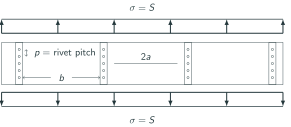
\includegraphics{../images/crack-under.svg}
\end{frame}

\begin{frame}{centered under stiffener}
\protect\hypertarget{centered-under-stiffener}{}
\includegraphics{../images/crack-between.svg}
\end{frame}

\begin{frame}{remote stress}
\protect\hypertarget{remote-stress}{}
\begin{itemize}
\tightlist
\item
  For displacement continuity, we know that
\end{itemize}

\[\left(\frac{PL}{AE}\right)_{Skin} = \left(\frac{PL}{AE}\right)_{Stiffener}\]

\begin{itemize}
\tightlist
\item
  Since \emph{L} is the same, we find
\end{itemize}

\[\frac{S}{E} = \frac{S_S}{E_S}\]

\begin{itemize}
\tightlist
\item
  Where the subscript \emph{S} indicates stiffener values, we can
  express the remote stress in the stiffener as
\end{itemize}

\[S_S = S \frac{E_S}{E}\]
\end{frame}

\begin{frame}{skin}
\protect\hypertarget{skin}{}
\begin{itemize}
\tightlist
\item
  The critical stress in the skin is determined the same way as it was
  in the residual strength chapter
\item
  The only exception is that the stiffener contributes to \$\beta\$
\end{itemize}

\[S_C = \frac{K_C}{\sqrt{\pi a} \beta}\]
\end{frame}

\begin{frame}{stiffener}
\protect\hypertarget{stiffener}{}
\begin{itemize}
\tightlist
\item
  The maximum stress in a stiffener will be increased near a crack
\item
  We represent the ratio of maximum force in stiffener to remote force
  with the Stiffener Load Factor, \emph{L}
\end{itemize}
\end{frame}

\begin{frame}{stiffener}
\protect\hypertarget{stiffener-1}{}
\[\small{\begin{aligned}
  L &= \frac{\text{max force in stiffener}}{\text{remote force applied to stiffener}}\\
  &= \frac{S_{S,max}A_S}{S_S A_S}\\
  &= \frac{S_{S,max}}{S \frac{E_S}{E}}\\
  L S \frac{E_S}{E} &= S_{S,max}\\
  L S \frac{E_S}{E} &= \sigma_{YS}\\
  S_C &= \frac{\sigma_{YS} E}{L E_S}
\end{aligned}}\]
\end{frame}

\begin{frame}{rivet}
\protect\hypertarget{rivet}{}
\begin{itemize}
\tightlist
\item
  We can define a similar rivet load factor to relate maximum stress in
  the rivet to remote stress in the skin
\end{itemize}

\[\begin{aligned}
  L_R &= \frac{\tau_{max} A_R}{S b t}\\
  L_R &= \frac{\tau_{YS} A_R}{S b t}\\
  S_c &= \frac{\tau_{YS} A_R}{L_R b t}
\end{aligned}\]
\end{frame}

\begin{frame}{finite element analysis}
\protect\hypertarget{finite-element-analysis}{}
\begin{itemize}
\tightlist
\item
  CC Poe found that panels could be related by a parameter he defines as
  \(\mu\)
\end{itemize}

\[\mu = \frac{A_S E_S}{A_S E_S + A E}\]

\begin{itemize}
\tightlist
\item
  Where \emph{A}\emph{S} is the cross-sectional area of a stiffener,
  \emph{E}\emph{S} is stiffener modulus
\item
  \emph{A} is the skin cross-sectional area (per stiffener)
  \emph{A}=\emph{bt} and \emph{E} is the modulus of the skin
\end{itemize}
\end{frame}

\begin{frame}{finite element analysis}
\protect\hypertarget{finite-element-analysis-1}{}
\begin{itemize}
\tightlist
\item
  pp 167 - 178 give \(\beta\), \emph{L} and \emph{L}\emph{R} for various
  skin/stiffener configurations
\item
  These values were determined using a finite element model
\end{itemize}
\end{frame}

\begin{frame}{examples}
\protect\hypertarget{examples}{}
\begin{itemize}
\tightlist
\item
  quantitative example (p.~179-180)
\item
  qualitative notes on behavior (p.~181-182)
\item
  \href{../examples/stiffener\%20example.html}{worked}
\end{itemize}
\end{frame}

\end{document}
